\documentclass{article}
\usepackage[margin=1in]{geometry}
\usepackage{amsmath}
\usepackage{graphicx}




\begin{document}

\title{\textbf{Airfoil Selection}}
\author{Abigail Gries}
\maketitle

Choosing an airfoil is an imperative preliminary step in the design of an unmanned aircraft system. UAS performance can be severely limited by an airfoil that is not appropriate. This document outlines the process and resources that the OpenUAS team used to select an airfoil. 

\section*{Step 1 - Researching Airfoil Candidates}

The team's UAS will be flying at low velocities and low Reynold's numbers due to budget, legal, and technological constraints. Research was first done to find potential airfoils that perform well at these conditions. Various resources were used to locate qualified airfoils, however, one academic paper proved to be very useful [1]. From this paper, three airfoils were selected: NACA 0015, NACA 0019, and NACA 4512. These specific airfoils were chosen because they had dominant airspeeds in the same range of our UAS (15 m/s to 30 m/s) and they performed well in the optimization process detailed in the paper [1]. 

\section*{Step 2 - XFLR5 Analysis}

XFLR5 is a tool that analyzes airfoils and generates relevant data about those airfoils. The three airfoils, NACA 0015, NACA 0019, and NACA 4512, were loaded into the program, and a direct foil analysis was performed on each candidate. The analysis performed was Type 1, with a Reynold's number of 100,000, Mach number of 0, and a Ncrit value of 9. The Reynold's number value was chosen based on the altitude of Ames, Iowa and the cruise speed at which the UAS will likely be flying. The Ncrit value was chosen to be 9 as this is a commonly used value for simulating normal turbulent flow. Data was generated for angles of attack ranging from -5 degrees to 15 degrees. Once the program completed the analysis for the three airfoils, the data produced was exported to csv files. 

\section*{Step 3 - Calculations}

Using the csv files created by XFLR5, two different plots were created for each airfoil. The coefficient of lift and the angle of attack were plotted against each other. From this graph, important characteristics of the airfoil could be determined. Specifically, the coefficient of zero lift drag, the maximum coefficient of lift, and the stall angle of attack were all estimated using the plots. The coefficient of zero lift drag, or $Cl_{0}$, was determined by finding the y-intercept of the  $Cl$ vs $\alpha$ plot. The maximum coefficient of lift, $Cl_{max}$, is the highest coefficient of lift in the given range of alpha, so the maximum peak of the curve was selected for each airfoil. The stall angle of attack, $\alpha_{stall}$, was estimated as the angle in degrees associated with the end of the linear range of each plot. Another plot was also created using the data from the csv files. The coefficient of lift vs coefficient of drag, or $Cl$ vs $Cd$, plot was produced, and from this plot, the minimum coefficient of drag and the maximum of efficiency of the airfoils were estimated. The minimum coefficient of drag, $Cd_{min}$, is the x-intercept of the $Cl$ vs $Cd$ plot. The maximum aerodynamic efficiency, or $E_{max}$, is the point with the highest slope on the plot. These characteristics of each airfoil, the coefficient of zero lift drag, the maximum coefficient of lift, the stall angle of attack, the minimum coefficient of drag, and the maximum aerodynamic efficiency, are all key parameters that were used in selecting the most appropriate airfoil for the OpenUAS project. The values for each parameter are shown in the table below.\\

\begin{figure}
\begin{center}
	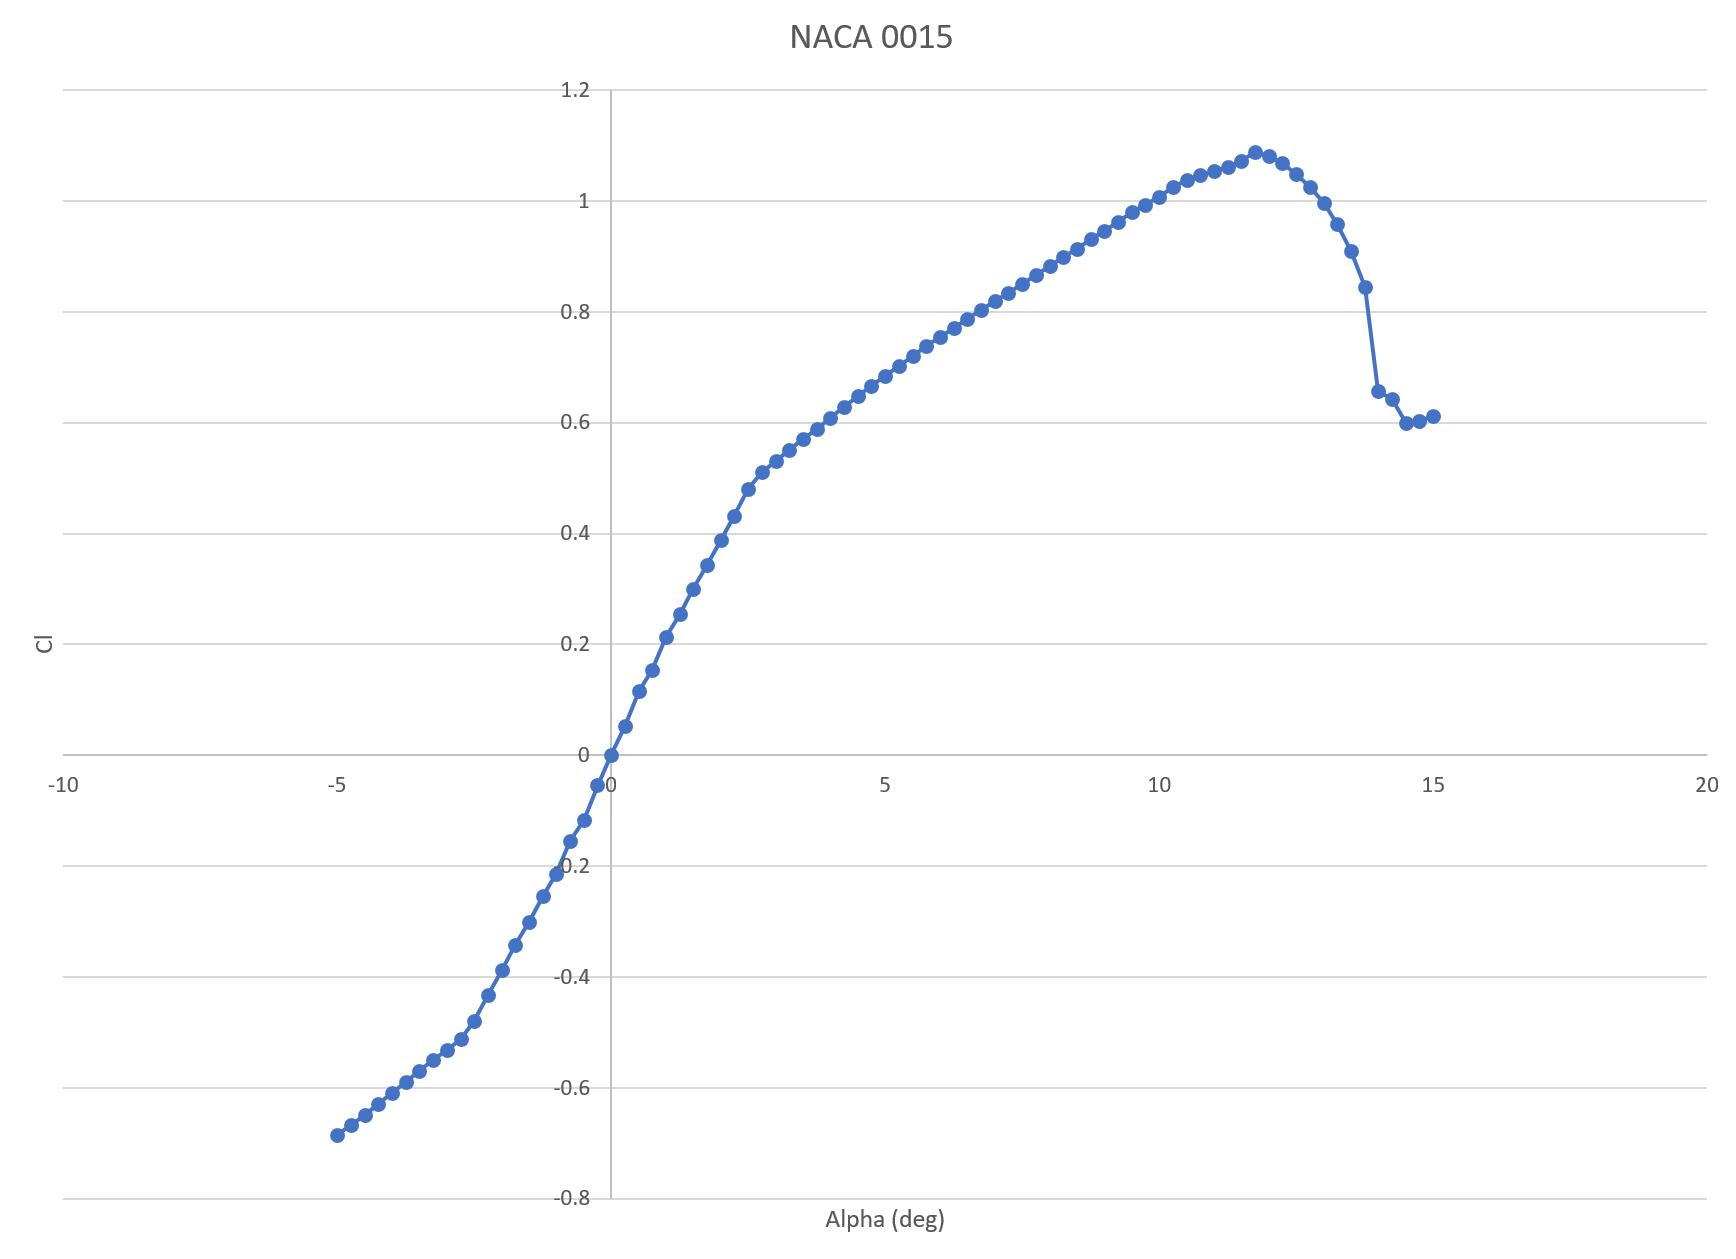
\includegraphics[scale=0.4]{NACA0015clvsalpha.png}
	\caption{NACA 0015 $Cl$ vs $\alpha$}
	\label{Figure 1:}

\end{center}
\end{figure}


\begin{figure}
\begin{center}
	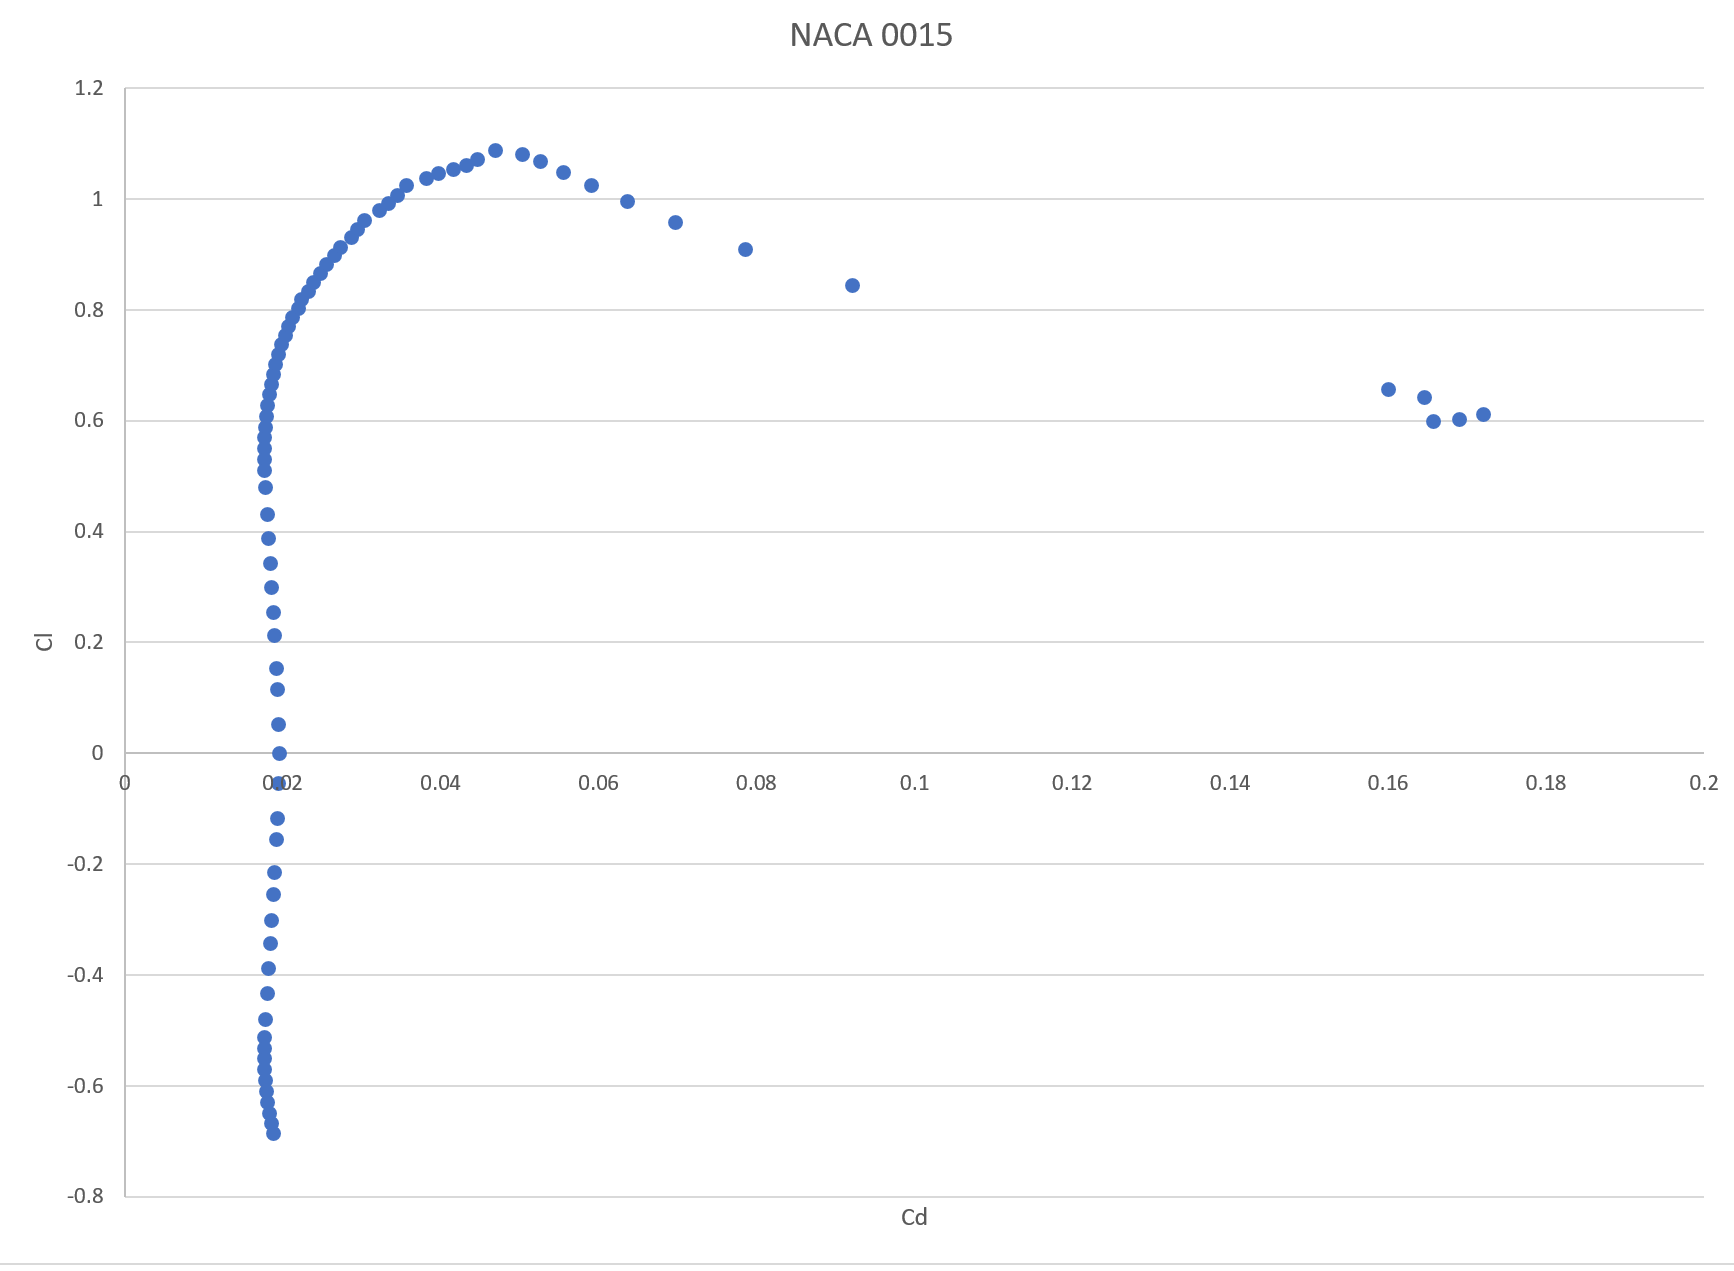
\includegraphics[scale=0.4]{NACA0015clvscd.png}
	\caption{NACA 0015 $Cl$ vs $Cd$}
	\label{Figure 2:}
\end{center}
\end{figure}

\begin{figure}
\begin{center}
	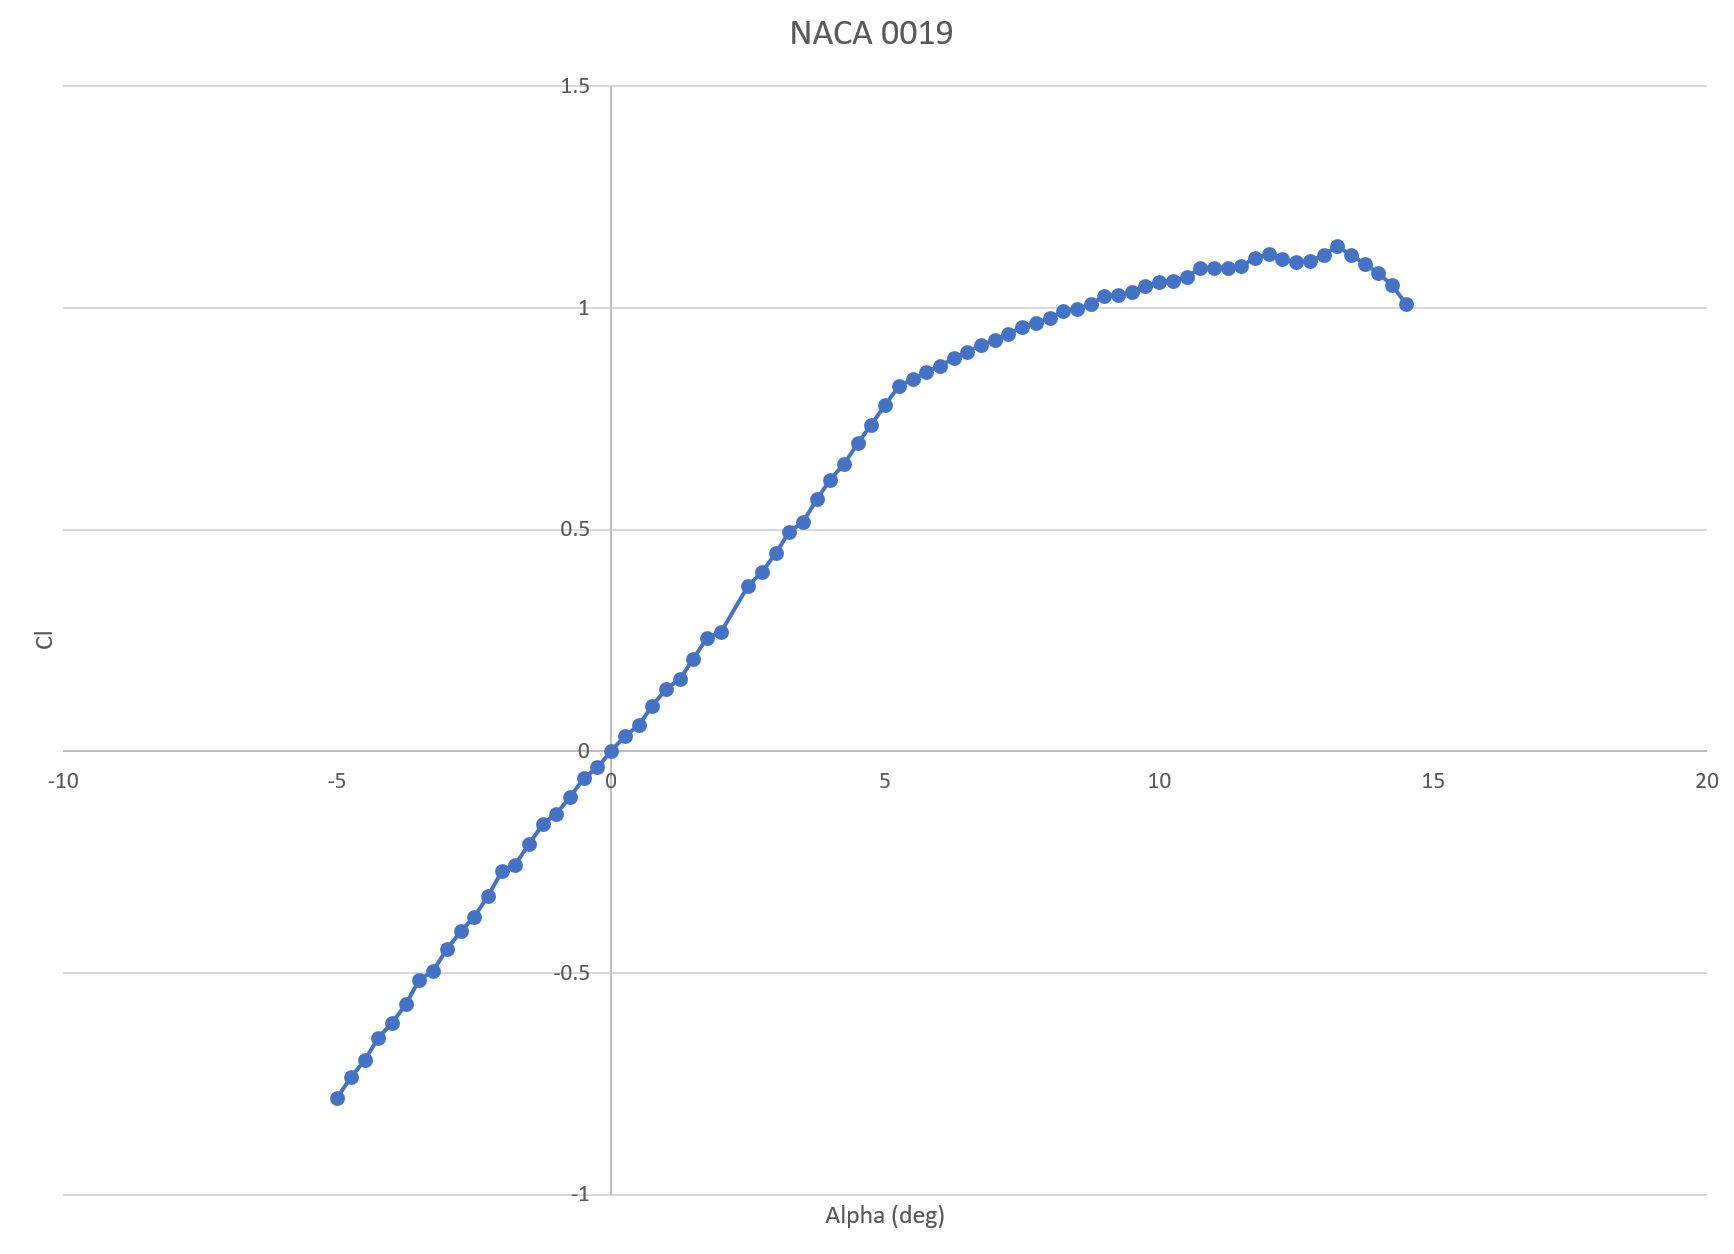
\includegraphics[scale=0.4]{NACA0019clvsalpha.png}
	\caption{NACA 0019 $Cl$ vs $\alpha$}
	\label{Figure 3:}

\end{center}
\end{figure}

\begin{figure}
\begin{center}
	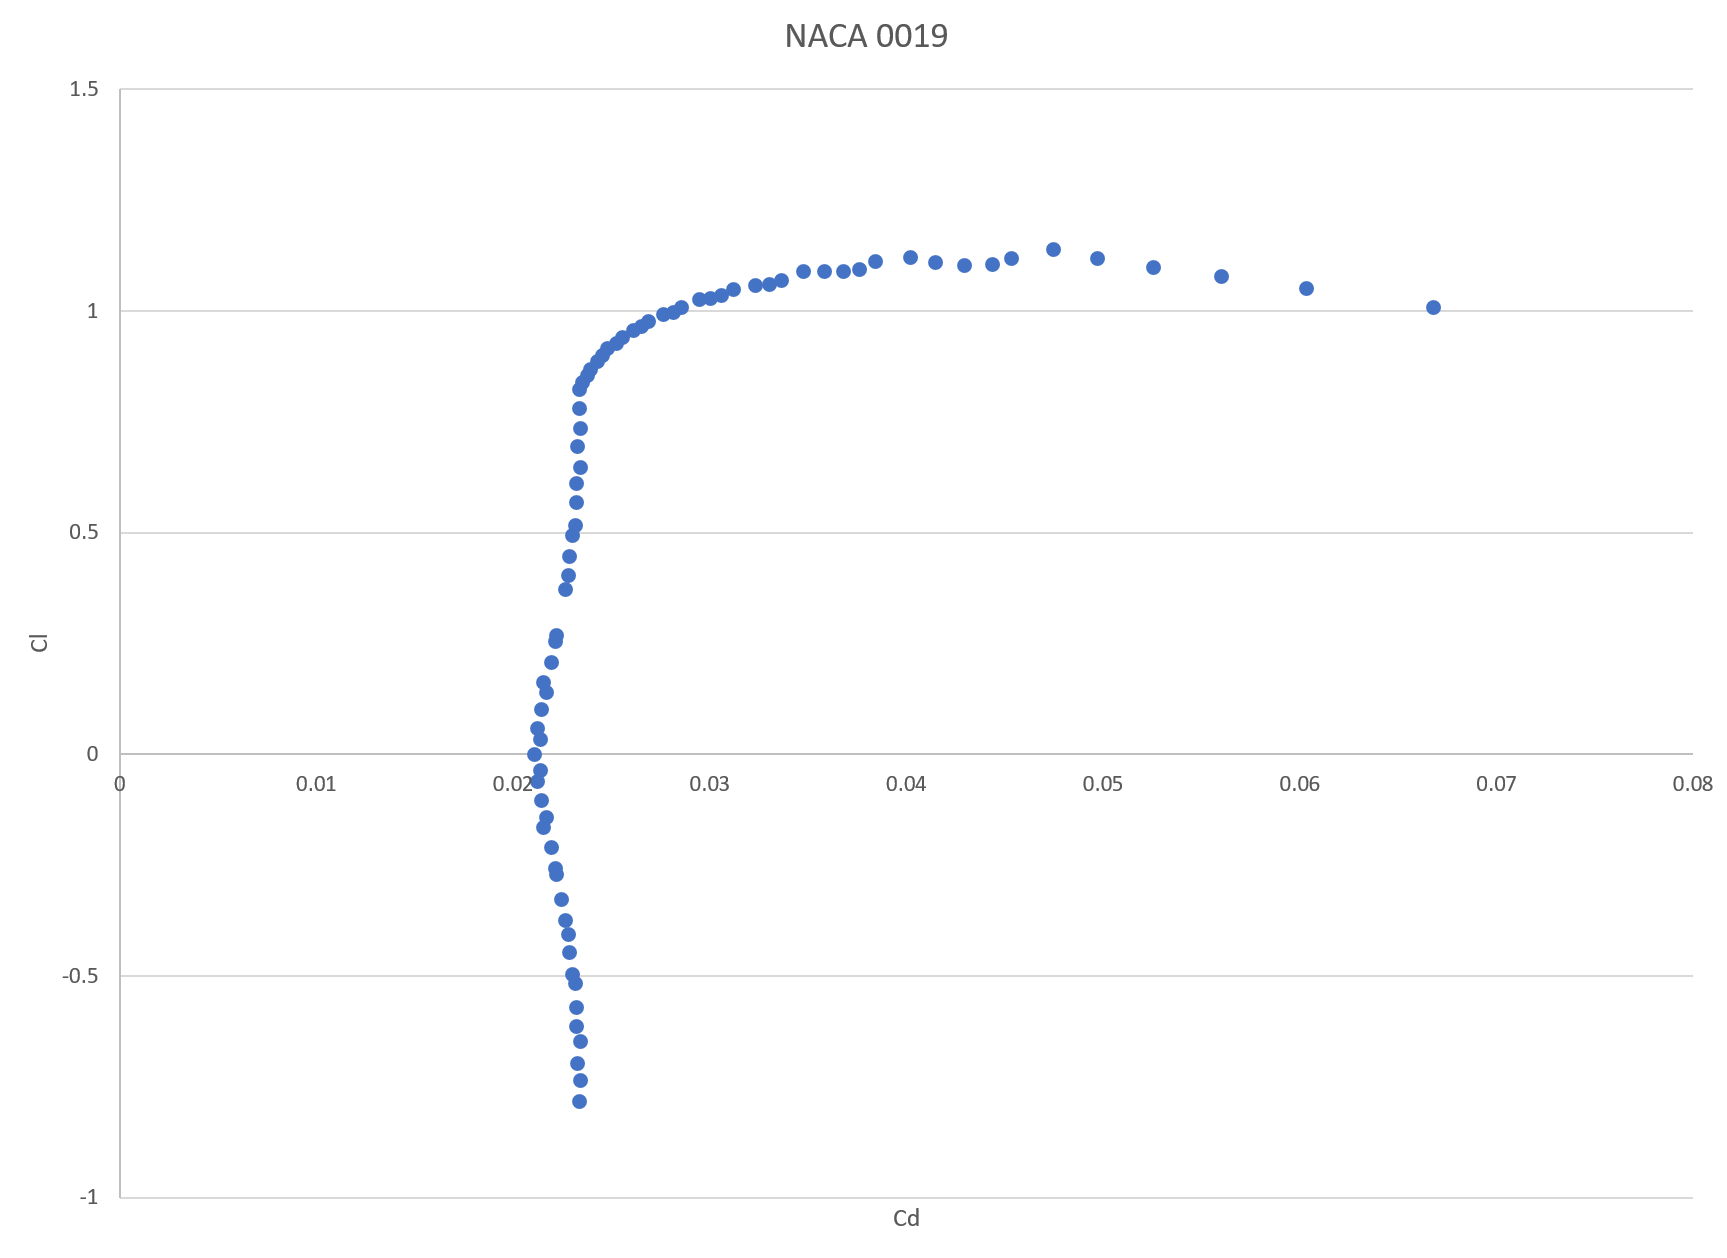
\includegraphics[scale=0.4]{NACA0019clvscd.png}
	\caption{NACA 0019 $Cl$ vs $Cd$}
	\label{Figure 4:}
\end{center}
\end{figure}

\begin{figure}
\begin{center}
	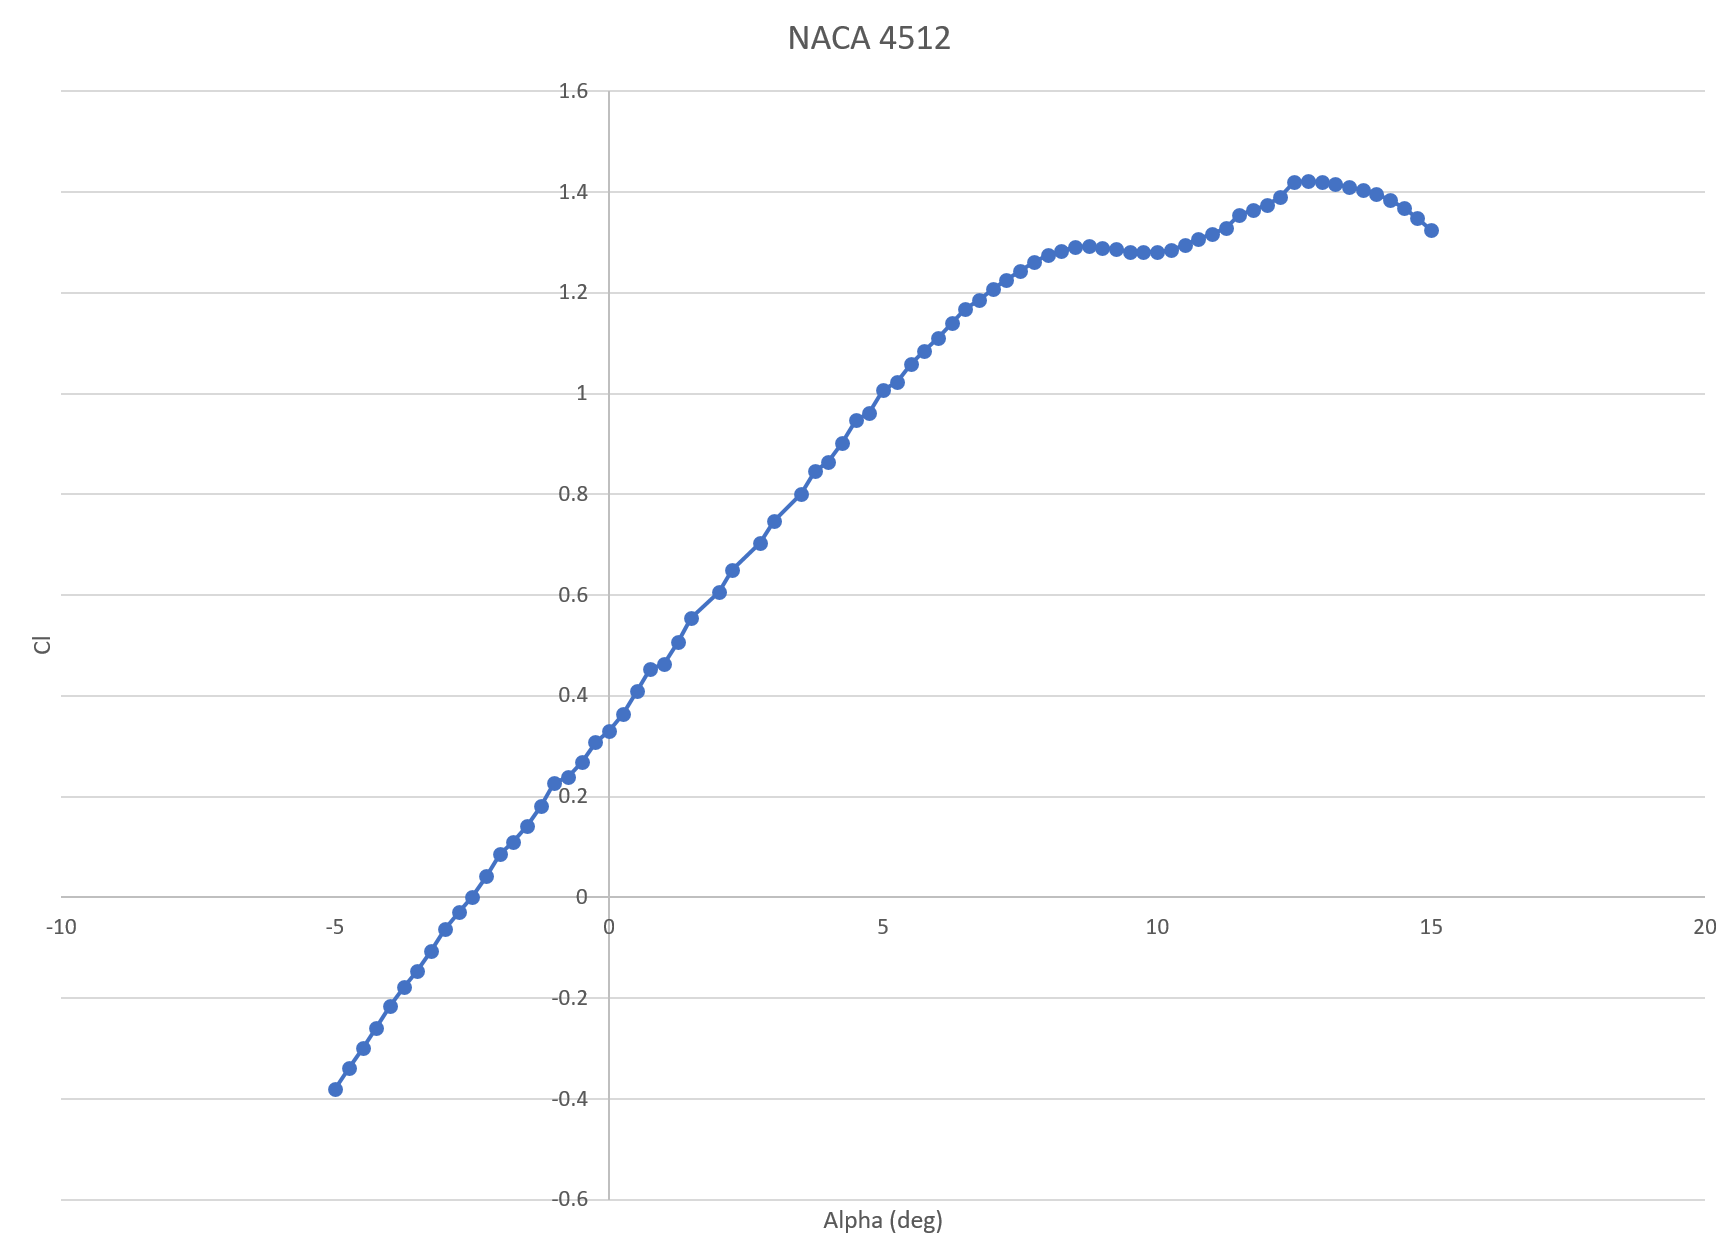
\includegraphics[scale=0.4]{NACA4512clvsalpha.png}
	\caption{NACA 4512 $Cl$ vs $\alpha$}
	\label{Figure 5:}
\end{center}
\end{figure}

\begin{figure}
\begin{center}
	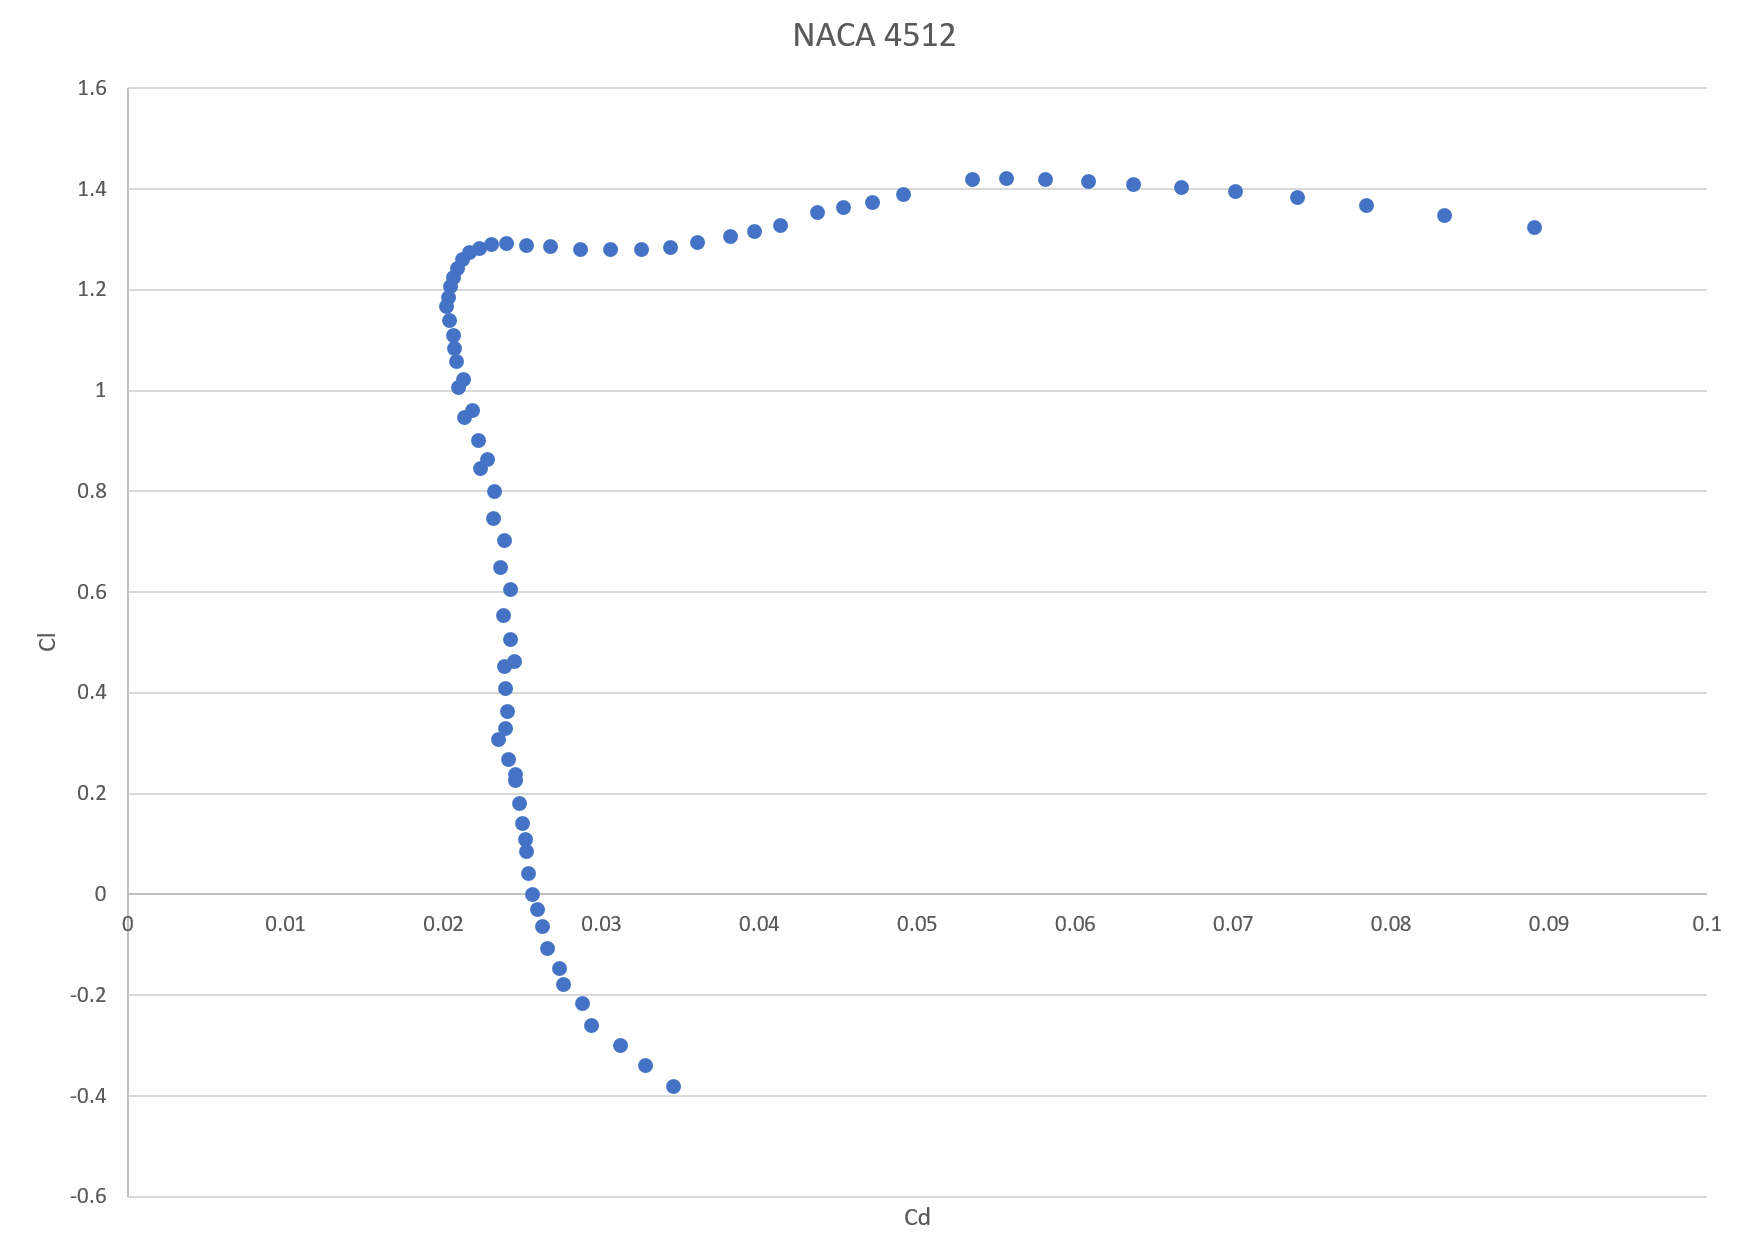
\includegraphics[scale=0.4]{NACA4512clvscd.png}
	\caption{NACA 4512 $Cl$ vs $Cd$}
	\label{Figure 6:}
\end{center}
\end{figure}
\begin{tabular}[pos]{| c | c | c | c |}


\hline
Parameter & NACA 0015 & NACA 0019 & NACA 4512 \\ \hline
$Cl_{0}$ & 0 & 0 & 0.3293   \\ \hline
$Cl_{max}$  & 1.0876 & 1.1212 & 1.2921  \\ \hline
$\alpha_{stall}$ & 10.25 & 9.75 & 7.25 \\ \hline
$Cd_{min}$ & 0.01948 & 0.02107 & 0.02562 \\ \hline
$E_{max}$ & 37.35 & 36.96 & 59.67 \\ \hline


\end{tabular}

\section*{Step 4 - Weighted Scoring Method}

In order to select the most appropriate airfoil based on the parameters outlined in the Calculations section, a weighted scoring method was used. This method is a modified version of the process used in reference [2]. A ranking place, 1st, 2nd, or 3rd, is given to each airfoil for each parameter. Each place has the following points associated with it: 3 points for 1st place, 2 points for 2nd place, and 1 point for 3rd place. Then, each parameter has a weight associated with it. The points an airfoil receives for each parameter are multiplied by the weight or "multiplier." Finally, all the weighted points are added up, and the airfoil with the highest point total is considered the best selection. The table below shows the ranking, multiplier, and total points for each airfoil. \\ \\

\begin{tabular}[pos]{| c | c | c | c | c | c |}


\hline
Parameter & Evaluation & NACA 0015 & NACA 0019 & NACA 4512 & Multiplier \\ \hline
$Cl_{0}$ & Closest to cruise is best & 2nd & 2nd & 1st & 1.2  \\ \hline
$Cl_{max}$ & Highest is best & 3rd & 2nd & 1st & 1.25 \\ \hline
$\alpha_{stall}$ & Highest is best & 1st & 2nd & 3rd & 1.15 \\ \hline
$Cd_{min}$ & Lowest is best & 1st & 2nd & 3rd & 1.15 \\ \hline
$E_{max}$ & Highest is best & 2nd & 3rd & 1st & 1.25  \\ \hline
Total Points & & \textbf{13.05} & \textbf{10.75} & \textbf{13.4} & \\ \hline


\end{tabular}


\section*{Step 5 - Selection}

The airfoil with the highest overall point total was NACA 4512. This airfoil was selected by the OpenUAS team as the airfoil to use on the first UAS design.


\section*{References}

[1] V. Brusov \& V. Petruchik. (2011). Design Approach for Selection of Wing Airfoil with Regard to Micro-UAVs. International Micro Air Vehicle Conference, Netherlands, September 2011. Delft University of Technology. Retreived from: https://repository.tudelft.nl/islandora/object/uuid:2b261a19-fae4-44dd-ac04-1113ebc7c89b?collection=research \\

\noindent [2] Ngo, Khanh \& Thien Loc, Huynh. (2016). Airfoil Selection for Fixed Wing of Small Unmanned Aerial Vehicles. 881-890. 10.1007/978-3-319-27247-4\_73.




\end{document}

